\documentclass[conference,a4paper]{IEEEtran}
\IEEEoverridecommandlockouts
\renewcommand\IEEEkeywordsname{Keywords}

\usepackage{flushend}
\usepackage{cite}
\usepackage{amsmath,amssymb,amsfonts}
\usepackage{graphicx}
\usepackage{textcomp}
\usepackage{xcolor}
\usepackage{listings}
\usepackage{booktabs}
\usepackage{url}
\usepackage{array}
\usepackage{tabularx}
\usepackage[utf8]{inputenc}

\lstset{
    language=C,
    basicstyle=\ttfamily\scriptsize,
    breaklines=true,
    frame=single,
    captionpos=b,
    keywordstyle=\color{blue},
    numbers=none,
    columns=fullflexible,
    keepspaces=true,
    xleftmargin=2pt,
    xrightmargin=2pt,
    aboveskip=3pt,
    belowskip=0pt
}

\begin{document}

% --- TITLE ---
\title{Empirical Analysis of Optimization Phase Ordering
Trade-offs in a Custom Compiler Using
Micro-Benchmarks}

\author{
    \makebox[\textwidth][c]{%
        \begin{minipage}[t]{0.29\textwidth}
            \centering
            \text{Aniket De}\\
            \textit{Dept. of Computer Science and Engineering}\\
            \textit{Sahyadri College of Engineering}\\
            \textit{\& Management}\\
            Mangaluru, India\\
            aniketde66\allowbreak@gmail\allowbreak.com
        \end{minipage}%
        \hfill
        \begin{minipage}[t]{0.29\textwidth}
            \centering
            \text{Kushal S M}\\
            \textit{Dept. of Computer Science and Engineering}\\
            \textit{Sahyadri College of Engineering}\\
            \textit{\& Management}\\
            Mangaluru, India\\
            mrkushalsm\allowbreak@gmail\allowbreak.com
        \end{minipage}%
        \hfill
        \begin{minipage}[t]{0.29\textwidth}
            \centering
            \text{Manas S}\\
            \textit{Dept. of Computer Science and Engineering}\\
            \textit{Sahyadri College of Engineering}\\
            \textit{\& Management}\\
            Mangaluru, India\\
            salianmanas\allowbreak@gmail\allowbreak.com
        \end{minipage}
    }\\[2ex]

    \makebox[\textwidth][c]{%
        \begin{minipage}[t]{0.29\textwidth}
            \centering
            \text{Vivek Neeralagi}\\
            \textit{Dept. of Computer Science and Engineering}\\
            \textit{Sahyadri College of Engineering}\\
            \textit{\& Management}\\
            Mangaluru, India\\
            vivekneeralagi\allowbreak@gmail\allowbreak.com
        \end{minipage}%
        \hfill
        \begin{minipage}[t]{0.33\textwidth}
            \centering
            \text{Suhas A Bhyratae}\\
            \textit{Dept. of Computer Science and Engineering}\\
            \textit{Sahyadri College of Engineering}\\
            \textit{\& Management}\\
            Mangaluru, India\\
            suhasabhyraatae.cs@sahyadri.edu.in
        \end{minipage}%
        \hfill
        \begin{minipage}[t]{0.29\textwidth}
            \centering
            \text{Harisha}\\
            \textit{Dept. of Computer Science and Engineering}\\
            \textit{Sahyadri College of Engineering}\\
            \textit{\& Management}\\
            Mangaluru, India\\
            harisha.cs@sahyadri.edu.in
        \end{minipage}
    }
}

\IEEEpubid{\makebox[\textwidth][l]{979-8-3195-4904-4/26/\$31.00~\copyright2026 IEEE}}

\maketitle

% --- ABSTRACT ---
\begin{abstract}
The phase ordering problem, the dependence of optimization results on the order in which compiler passes are applied, is a long-standing issue in compiler design. This paper reports an exhaustive study of the problem on a purpose-built compiler with a handwritten lexical analyzer, a recursive-descent parser, and a Three-Address Code (3AC) intermediate representation, in which six classical passes (Constant Folding, Dead Code Elimination, Common Subexpression Elimination, Copy Propagation, Strength Reduction, and Algebraic Simplification) are independent, reorderable units under a configurable pass manager. All 720 orderings of the six passes were applied to fifteen micro-benchmarks adapted from MiBench and PolyBench/C, giving 10,800 optimized programs, each verified to print the same output as its unoptimized baseline. Static instruction count, an estimated cycle cost under a stated per-instruction cost model, and the dynamic instruction count from an IR interpreter were recorded. The best family of orderings reduces code size by a geometric mean of 35.7\% (22\% to 60\% per program), estimated cycles by 20.5\%, and executed instructions by 23.2\%, whereas a third of all orderings reduce code size by only 1.3\%. The 720 orderings collapse into nine equivalence classes fixed by the relative order of four passes, the same relative order is optimal on every program, and the effect is significant across programs (Friedman test, $p < 10^{-48}$, Kendall's $W = 0.88$).
\end{abstract}

\begin{IEEEkeywords}
Common Subexpression Elimination,
Compiler Optimization,
Constant Folding,
Dead Code Elimination,
Micro-Benchmarking,
Phase Ordering Problem,
Three-Address Code
\end{IEEEkeywords}

\vfill
\newpage

\section{Introduction}
\IEEEpubidadjcol

Compilers translate high-level languages into machine code, and the quality of that code determines execution speed, memory use, and energy \cite{ref21,ref18}. Optimizations such as Constant Folding, Dead Code Elimination, and Common Subexpression Elimination remove redundant work without changing program behaviour \cite{ref18}, but how much they remove depends on the order in which they run \cite{ref19}. This is the \textit{Phase Ordering Problem} \cite{ref1,ref2}: some passes expose opportunities for others while some destroy them, and the number of orderings grows factorially with the number of passes, so exhaustive evaluation is impractical in production compilers \cite{ref2}. LLVM and GCC therefore use fixed, heuristically tuned pipelines \cite{ref16}, which work well in practice but are too tightly coupled to isolate the effect of a single ordering decision.

This paper takes the opposite approach. It uses a small compiler in which six classical passes are implemented so that each is valid in any position, and it measures every one of the $6! = 720$ orderings on fifteen micro-benchmarks adapted from MiBench \cite{ref32} and PolyBench/C \cite{ref31}. Each configuration is measured by static instruction count (code size), an estimated cycle cost (a static model of runtime), and the number of instructions executed by an IR interpreter.

The six passes are textbook transformations \cite{ref18,ref21}; the contribution is the measurement, not the passes. Specifically: (1) an infrastructure in which every pass is block-local and side-effect free, so that all 720 orderings can be compared without a correctness caveat; (2) an exhaustive, output-validated evaluation of all orderings on fifteen kernels under three metrics; (3) the empirical structure of the ordering space, namely nine equivalence classes, four ordering rules, and a quantified cost of a poor order; and (4) a full specification of the metrics, cost model, and interaction-matrix derivation, with the source released\footnote{\url{https://github.com/VivekNeer/major-project-compiler-design}}, so that every table in the paper can be regenerated with one command.

\section{Related Work}

\textbf{Dependency modeling and pruning.} Liu et al. model dependences between passes to avoid redundant transformations \cite{ref1}, and Huemer et al. prune low-impact transformations to cut compilation time \cite{ref4}. Both rely on heuristics and on structural assumptions about the pass set.

\textbf{Machine learning.} Learned models select passes from program features: POSET-RL uses reinforcement learning to trade code size against execution time \cite{ref8}, AutoPhase learns phase orders for high-level synthesis \cite{ref12}, and MiCOMP learns over optimization subsequences \cite{ref15}. Related work includes program embeddings \cite{ref9}, predictive and ensemble models for flag or phase selection \cite{ref17,ref22,ref28,ref29}, graph-based iterative pass selection \cite{ref20}, and methods that enlarge or restructure the search space through dormant information \cite{ref2,ref26}, booster pass chains \cite{ref25}, or search for globally optimal code \cite{ref3}. These methods improve search efficiency but add training overhead and depend on large datasets \cite{ref8,ref12,ref15}.

\textbf{Production frameworks.} LLVM introduced a modular IR that supports continuous transformation and analysis \cite{ref16}; within such compilers, run-time data \cite{ref23}, comparison of optimization decisions \cite{ref24}, compilation statistics \cite{ref7}, and agile pass pipelines \cite{ref27} have been used to steer optimization. Their pipelines are tightly coupled, which makes pass interactions hard to isolate in a controlled setting \cite{ref16}.

\textbf{Gap.} Most of the work above optimizes for performance and treats the pipeline as a black box. Kulkarni et al. observed that many phase sequences produce identical code and that, for a small pass set, the distinct outcomes can be enumerated exhaustively \cite{ref19}; this study relies on exactly that property. Visualization tools for teaching optimizations \cite{ref30} address transparency but do not measure ordering effects. Table~\ref{tab:lit_review} summarizes the gap addressed here: a small infrastructure in which the trade-off between performance and code size can be measured, rather than estimated, for a given set of passes.

\begin{table}[htbp]
\caption{Comparative Analysis of Related Work}
\label{tab:lit_review}
\centering
\renewcommand{\arraystretch}{1.1}
{\small
\begin{tabularx}{\columnwidth}{@{}p{0.2\columnwidth} p{0.24\columnwidth} X@{}}
\toprule
\textbf{Reference} & \textbf{Focus Area} & \textbf{Limitation addressed by this work} \\
\midrule
Liu et al. \cite{ref1} & Pass-dependency modeling & Targets large compilers; no lightweight experimental framework. \\
Han \& Kim \cite{ref2} & Expanded search strategies & Increases complexity and reduces interpretability. \\
Ashouri et al. \cite{ref15} & ML-guided subsequences & Needs large datasets and extensive feature engineering. \\
\bottomrule
\end{tabularx}
}
\end{table}

\section{Compiler Infrastructure}

\subsection{Architecture and Intermediate Representation}
The compiler (Fig.~\ref{fig:architecture}) is a pipeline of independent modules: a handwritten lexer produces tokens with positions; a recursive-descent parser builds an abstract syntax tree; a semantic analyzer checks declarations, arity, and array use; an IR generator lowers the tree to 3AC; a pass manager applies optimizations in any requested order; and an interpreter executes the IR, counts executed instructions, and captures printed output. The source language is a C subset with integers, one-dimensional arrays, functions, \texttt{while}, \texttt{if}, and \texttt{print}. 3AC was chosen because each instruction has at most one operator and two operands, which keeps the local analyses the passes need (use and definition sets, an available-expression table) short and readable. The IR has 35 opcodes, seven of which (labels, no-ops, function markers, parameter declarations, array and global declarations) are structural and produce no machine code. A RISC-V RV32IM back end is included and is used only to confirm that size reductions measured on the IR survive code generation.

\begin{figure}[htbp]
    \centering
    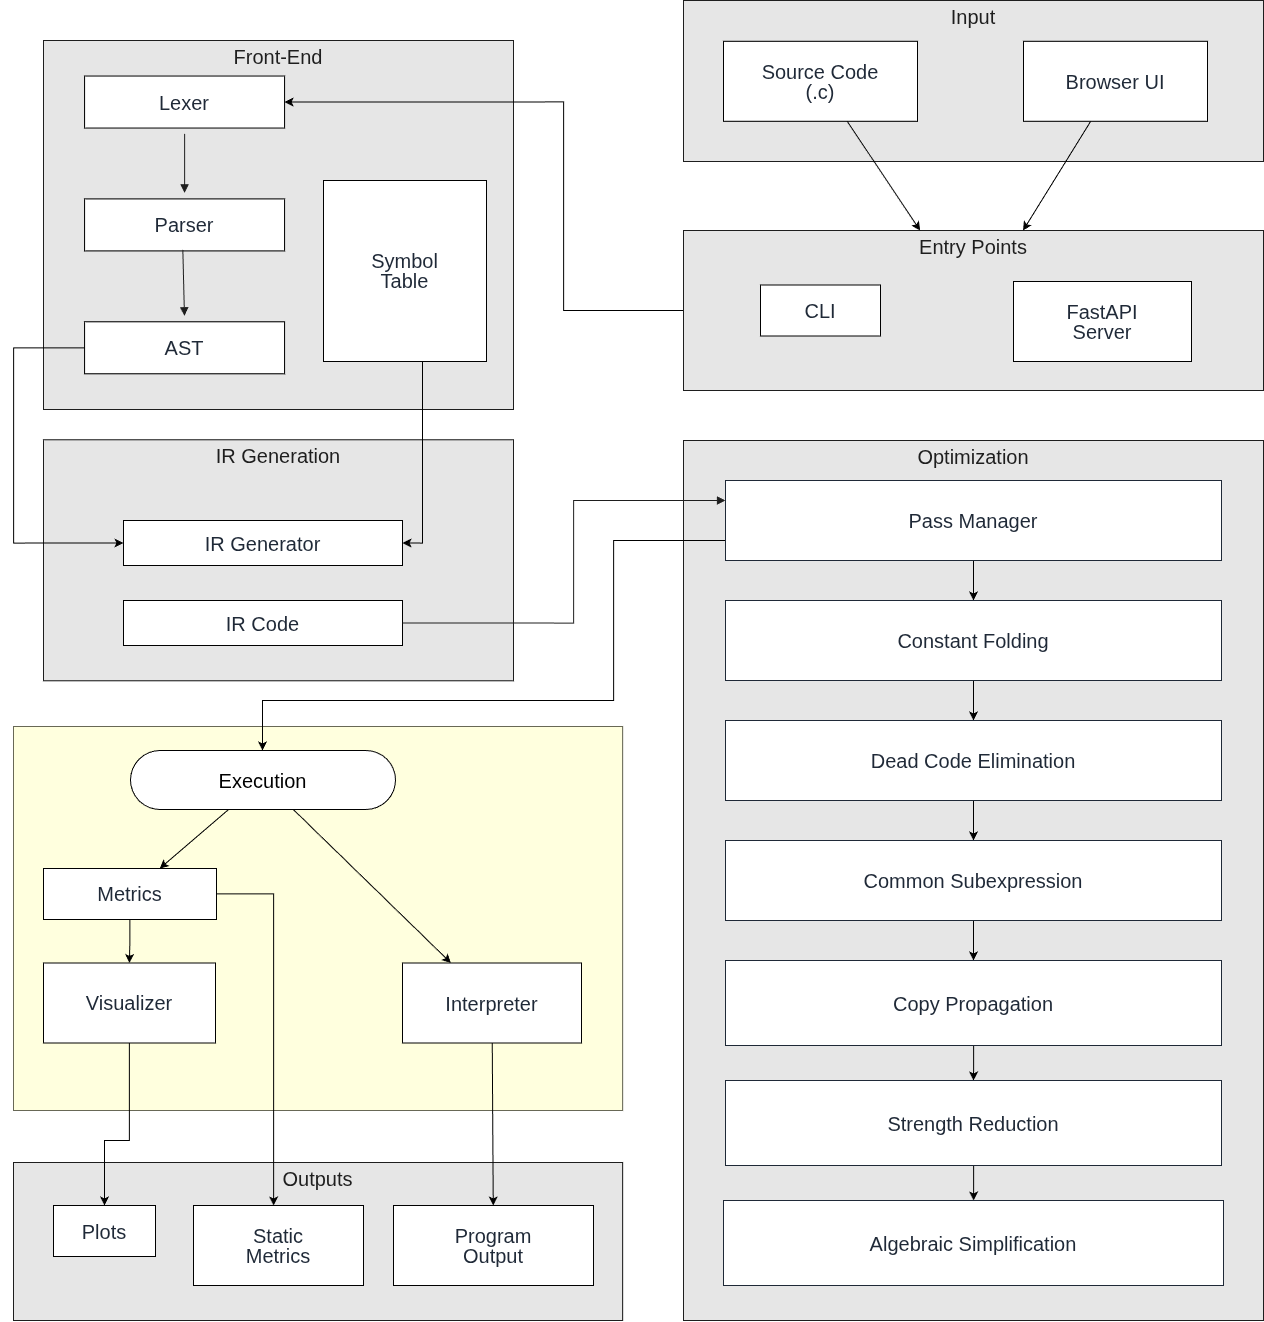
\includegraphics[width=0.72\linewidth]{fig/arc.png}
    \caption{Component-based architecture of the compiler: compilation pipeline and optimization framework.}
    \label{fig:architecture}
\end{figure}

\subsection{Optimization Passes}
\label{sec:passes}
Six passes are implemented, each as a function from an instruction list to a new list. All six are \emph{block-local}: each walks the list once or to a fixed point and discards every accumulated fact at each label, jump, call, and function boundary. This classical basic-block restriction makes the passes weaker than global versions, but it makes the correctness of each pass independent of what ran before it, which is what permits arbitrary reordering. No pass mutates its input.
\begin{itemize}
    \item \textbf{Constant Folding (CF):} a variable defined exactly once by a constant load, or by a copy of a known constant, enters a constant map; constants are substituted into operands and any arithmetic, comparison, or logical instruction with two constant operands becomes a constant load, repeated to a fixed point. A conditional jump on a constant becomes a jump or a no-op. Stores are never removed.
    \item \textbf{Dead Code Elimination (DCE):} deletes instructions after an unconditional jump or return up to the next label, then repeatedly deletes any side-effect-free instruction whose result is never read. Prints, returns, calls, parameter pushes, jumps, labels, and stores are never deleted.
    \item \textbf{Common Subexpression Elimination (CSE):} a table keyed by (opcode, operand, operand) records the variable holding each value; a repeated key becomes a copy from the earlier result. Redefinition of an operand or result invalidates the affected entries. Array loads are excluded because an intervening store may change the element.
    \item \textbf{Copy Propagation (CP):} a map from copied variables to their sources, resolved transitively, replaces later uses; constant loads also enter the map. An entry is dropped when either side is redefined.
    \item \textbf{Strength Reduction (SR):} single-instruction rewrites such as $x \times 2 \to x + x$, $x \times 1 \to$ copy, $x \times 0 \to 0$, $x / 1 \to$ copy, and $x - x \to 0$. SR never changes the instruction count; it changes the estimated cycle cost and may create copies for CP and DCE.
    \item \textbf{Algebraic Simplification (AS):} folds negation or logical-not of constants, self-comparisons ($x = x \to 1$, $x \neq x \to 0$), $x \wedge 0 \to 0$, and $x \vee k \to 1$ for non-zero constant $k$. AS never changes the instruction count.
\end{itemize}
The pass manager validates a requested ordering, folds a copy of the input IR through the passes in order, records the IR after each pass, and can enumerate all 720 permutations, which with the baseline give 721 configurations per program.

\subsection{Metrics and Cost Model}
\label{sec:metrics}
\textit{Static code size} is the number of IR instructions excluding labels, no-ops, function markers, parameter declarations, and global declarations (an array declaration counts as one instruction but costs zero cycles). \textit{Estimated execution cycles} is the sum over those instructions of a per-opcode cost from Table~\ref{tab:cost_model}: approximate latencies for an ARM Cortex-M class in-order core, the kind of target MiBench represents. The model is static, counts each instruction once regardless of execution frequency, and ignores caches, pipelines, and branch prediction; it is a weighting of code size by instruction class, not a prediction of wall-clock time. \textit{Dynamic instruction count} is the number of IR instructions the interpreter executes on the program's fixed input; it is independent of the cost model and is the model-free proxy for runtime. All percentages are reductions from the same program's baseline, $100 (1 - m_{\mathrm{opt}}/m_{\mathrm{base}})$, and all normalized values are the ratio $m_{\mathrm{opt}}/m_{\mathrm{base}}$ (1.0 = baseline, smaller is better).

\begin{table}[!htbp]
\centering
\caption{Per-instruction cost model for the estimated-cycle metric}
\label{tab:cost_model}
\renewcommand{\arraystretch}{1.05}
{\footnotesize
\begin{tabularx}{\columnwidth}{@{}>{\raggedright\arraybackslash}Xc@{}}
\toprule
\textbf{IR opcodes} & \textbf{Cost} \\
\midrule
ADD, SUB, NEG, comparisons, AND, OR, NOT, COPY, LOAD\_CONST, PARAM & 1 \\
MUL & 3 \\
DIV, MOD & 12 \\
JUMP, JUMP\_IF\_TRUE, JUMP\_IF\_FALSE & 2 \\
ARR\_LOAD, ARR\_STORE, GLOBAL\_LOAD, GLOBAL\_STORE & 2 \\
CALL / RETURN / PRINT & 5 / 3 / 10 \\
LABEL, NOP, FUNC\_BEGIN, FUNC\_END, FUNC\_PARAM, ARR\_DECL, GLOBAL\_DECL & 0 \\
\bottomrule
\end{tabularx}
}
\end{table}

\section{Experimental Method}
\label{sec:setup}

\textbf{Environment and procedure.} The compiler is pure Python; the analysis scripts use NumPy and Matplotlib. All results were produced on one machine (AMD Ryzen 7 7435HS, 24 GB RAM, Linux Mint 22.2, Python 3.12.3, NumPy 1.26.4, Matplotlib 3.11.0). The compiler uses no randomness, timing, or floating-point arithmetic in any decision, so repeated runs on any machine give identical IR and metric tables. For each program the baseline IR is generated once; each of the 720 orderings is applied to a copy, measured, executed, and its printed output compared with the baseline's. The whole experiment, 10,815 compile-and-execute runs, is one command (\texttt{python -m compiler.main --benchmark-all}) and takes 23.5 s.

\textbf{Benchmark suite.} Fifteen programs were adapted from MiBench \cite{ref32} and PolyBench/C \cite{ref31} kernels (Table~\ref{tab:per_program}). The eight MiBench-derived programs are scalar (loops, conditionals, calls, division and modulo); the seven PolyBench-derived programs are array-based (stencils and matrix kernels with flattened row-major indexing). Bit operations are written as division and modulo by two, floating-point kernels are made integer, two-dimensional arrays are flattened with explicit index arithmetic, and inputs are fixed to small constant sizes ($4\times4$ or $5\times5$ matrices, vectors of 5 or 8) with results printed so that the output is a complete witness of the computation. Two programs (\texttt{factorial}, \texttt{sha\_mix}) contain planted dead code and repeated subexpressions; the other thirteen contain no planted opportunities.

\textbf{Statistical analysis.} Because the compiler is deterministic there is no run-to-run variance, and because all 720 orderings are enumerated there is no sampling of orderings. Inference therefore concerns one question: does the ordering effect generalize across programs? Three tests use programs as the unit of replication: a Friedman test with the fifteen programs as blocks and the 24 relative orders of CF, CSE, CP, and DCE as treatments (SR and AS do not affect size, Section~\ref{sec:classes}), with Kendall's $W$ as effect size; an exact Wilcoxon signed-rank test between the best and worst classes, with the matched-pairs rank-biserial $r$; and Spearman's $\rho$ between metrics. Cross-program aggregates use the geometric mean of per-program ratios \cite{ref33}.

\section{Results and Discussion}
Sections~\ref{sec:factorial} and~\ref{sec:interaction} follow one program, \texttt{factorial}, whose size allows every number to be checked by hand; Sections~\ref{sec:classes} to~\ref{sec:validation} cover all fifteen programs and all 720 orderings.

\subsection{Worked Example: the Factorial Benchmark}
\label{sec:factorial}
Listing~\ref{lst:factorial} shows the source, written to contain constant expressions (\texttt{base}, \texttt{extra}), dead assignments (\texttt{unused}, \texttt{also\_unused}), and a repeated subexpression (\texttt{base + extra}). The IR generator places every literal in a temporary (\texttt{t6 = 2; t7 = 3; t8 = t6 + t7; base = t8}), so the unoptimized IR is larger than the source suggests. Its 40 countable instructions are 11 constant loads, 11 copies, 5 additions, 2 multiplications, 1 subtraction, 1 comparison, 2 jumps, 1 parameter push, 1 call, 2 returns, and 3 prints (13 in \texttt{factorial}, 27 in \texttt{main}), costing $30 + 2 \times 3 + 2 \times 2 + 5 + 2 \times 3 + 3 \times 10 = 81$ estimated cycles under Table~\ref{tab:cost_model}. The best ordering leaves the loop in \texttt{factorial} at 10 instructions and reduces \texttt{main} to 6 (\texttt{param 5; t12 = call factorial; print t12; print 10; print 10; return 0}): 16 instructions, 55 cycles.

\begin{lstlisting}[caption={The \texttt{factorial} benchmark (comments removed).},label={lst:factorial}]
int factorial(int n) {
  int result = 1; int i = 1;
  while (i <= n) { result = result * i; i = i + 1; }
  return result;
}
int main() {
  int base = 2 + 3;  int extra = 10 - 5;
  int val = factorial(base);  print(val);
  int unused = 42 * 2;  int also_unused = unused + 100;
  int sum1 = base + extra;  int sum2 = base + extra;
  print(sum1);  print(sum2);  return 0;
}
\end{lstlisting}

Table~\ref{tab:phase_order_tradeoff} lists the baseline and six orderings. The 720 orderings produce exactly six distinct outcomes on this program, and the six sequences were chosen so that each appears once; AS is omitted because it never changes the instruction count, and appending it leaves every entry unchanged. The per-pass log shows where the reduction happens: under Seq~1 the size stays at 40 through CF, CSE, and CP and drops to 16 at DCE. The enabling passes remove nothing themselves; they replace instructions by equivalents (a folded expression becomes a constant load, a recomputation becomes a copy, an operand is renamed) that leave other instructions unread, and DCE deletes those. Run first, DCE finds only the seven planted dead instructions and the ordering ends at 33 (Seq~6); run after CF but before CSE and CP, it ends at 21 (Seq~4).

\begin{table}[!htbp]
\centering
\caption{Phase ordering on \texttt{factorial}: absolute metrics and percentage reduction from the baseline (40 instructions, 81 est.\ cycles, 81 executed)}
\label{tab:phase_order_tradeoff}
\renewcommand{\arraystretch}{1.1}
{\footnotesize
\setlength{\tabcolsep}{2.6pt}
\begin{tabular}{@{}llccccc@{}}
\toprule
 & & \multicolumn{2}{c}{\textbf{Absolute}} & \multicolumn{3}{c}{\textbf{Reduction (\%)}} \\
\cmidrule(lr){3-4}\cmidrule(lr){5-7}
\textbf{Label} & \textbf{Sequence} & Size & Cyc. & Size & Cyc. & Dyn. \\
\midrule
Base  & none & 40 & 81 & 0 & 0 & 0 \\
Seq 1 & CF $\to$ CSE $\to$ CP $\to$ DCE $\to$ SR & 16 & 55 & 60.0 & 32.1 & 34.6 \\
Seq 2 & CSE $\to$ CP $\to$ CF $\to$ DCE $\to$ SR & 18 & 57 & 55.0 & 29.6 & 32.1 \\
Seq 3 & CP $\to$ CF $\to$ DCE $\to$ CSE $\to$ SR & 19 & 58 & 52.5 & 28.4 & 30.9 \\
Seq 4 & CF $\to$ DCE $\to$ CSE $\to$ CP $\to$ SR & 21 & 60 & 47.5 & 25.9 & 28.4 \\
Seq 5 & CP $\to$ DCE $\to$ CF $\to$ CSE $\to$ SR & 22 & 61 & 45.0 & 24.7 & 27.2 \\
Seq 6 & DCE $\to$ CF $\to$ CSE $\to$ CP $\to$ SR & 33 & 72 & 17.5 & 11.1 & 8.6 \\
\bottomrule
\end{tabular}
}
\end{table}

\subsection{Pairwise Pass Interactions}
\label{sec:interaction}
Table~\ref{tab:pass_interaction} is computed from all 720 orderings on \texttt{factorial}, not from the six sequences above. For each ordered pair $(A, B)$ the entry is the mean static code size, in IR instructions, over the 360 orderings with $A$ before $B$ minus the mean over the 360 with $B$ before $A$; negative means the row pass should precede the column pass, and the matrix is antisymmetric by construction. The CF and CP rows against the DCE column carry the largest effects: CF before DCE saves 10.7 instructions out of 40 on average, CP before DCE saves 10.2. The matrix is a marginal statistic that averages over the positions of the other four passes, so an entry is not a causal effect of the pair alone: the AS and SR rows are non-zero although neither pass ever changes the instruction count, because in the population of orderings ``AS before CF'' is correlated with ``DCE relatively later''. The class analysis in Section~\ref{sec:classes}, which holds the other passes fixed, is the tool for attribution. Fig.~\ref{fig:pass_interaction} shows the same matrix as a heatmap, rounded to integers.

\begin{table}[!htbp]
\centering
\caption{Pairwise interaction matrix for \texttt{factorial}: mean code size with row pass before column pass minus the reverse (IR instructions, 720 orderings)}
\label{tab:pass_interaction}
\renewcommand{\arraystretch}{1.1}
{\footnotesize
\begin{tabularx}{\columnwidth}{@{}Xcccccc@{}}
\toprule
\textbf{A before B} & \textbf{AS} & \textbf{CF} & \textbf{CP} & \textbf{CSE} & \textbf{DCE} & \textbf{SR} \\
\midrule
AS  & 0      & $+$2.9 & $+$2.2 & $+$0.1 & $-$5.2  & 0 \\
CF  & $-$2.9 & 0      & $-$1.2 & $-$2.8 & $-$10.7 & $-$2.9 \\
CP  & $-$2.2 & $+$1.2 & 0      & $-$2.0 & $-$10.2 & $-$2.2 \\
CSE & $-$0.1 & $+$2.8 & $+$2.0 & 0      & $-$5.3  & $-$0.1 \\
DCE & $+$5.2 & $+$10.7 & $+$10.2 & $+$5.3 & 0     & $+$5.2 \\
SR  & 0      & $+$2.9 & $+$2.2 & $+$0.1 & $-$5.2  & 0 \\
\bottomrule
\end{tabularx}
}
\end{table}

\begin{figure}[htbp]
    \centering
    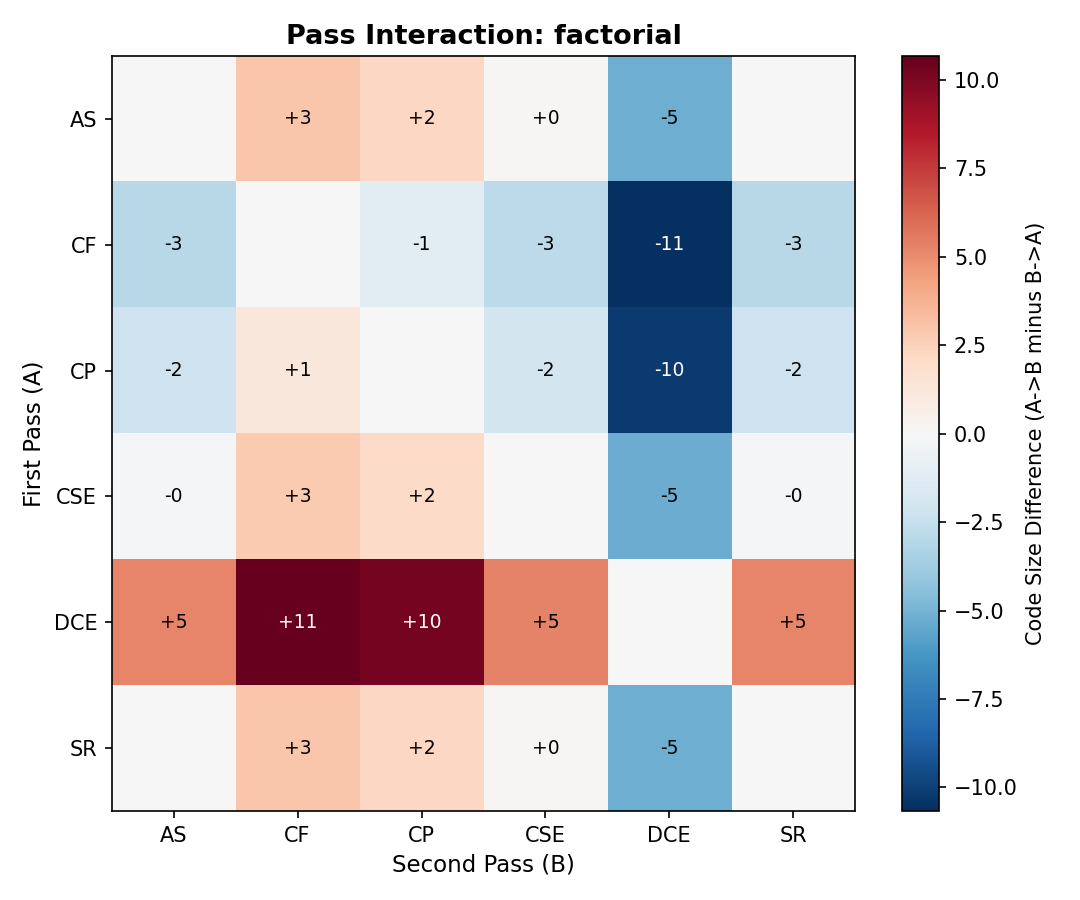
\includegraphics[width=0.78\columnwidth]{fig/factorial_pass_interaction.png}
    \caption{Heatmap of Table~\ref{tab:pass_interaction}: code size difference when applying pass A before pass B versus the reverse order.}
    \label{fig:pass_interaction}
\end{figure}

\subsection{Generalization Across Fifteen Benchmarks}
\label{sec:classes}
Table~\ref{tab:per_program} gives, for every program, the baseline and best static size, the reduction in all three metrics under the best ordering, and how many of the 720 orderings reach the best size. The best ordering has the same relative order of the four size-relevant passes, CF $\to$ CSE $\to$ CP $\to$ DCE, on every program, and it minimizes all three metrics simultaneously on every program. Across the suite it reduces code size by a geometric mean of 35.7\%, estimated cycles by 20.5\%, and executed instructions by 23.2\%. The scalar MiBench-derived programs are reduced by 33\% to 60\% in size, the array-based PolyBench-derived programs by 22\% to 34\%: in scalar kernels much of the baseline is literal-holding temporaries and copies that CF and CP make unread and DCE removes, whereas array kernels are dominated by loads and stores, which are never deleted without alias analysis, and by index arithmetic on loop-carried variables, which are not constant-propagation candidates. Cycle reductions are smallest on the division-heavy \texttt{power} and \texttt{gcd}, because division costs twelve cycles and its loop-carried operands keep it from being removed. Fig.~\ref{fig:box} shows the distribution of size reduction over all 720 orderings: the lower whisker reaches zero on thirteen programs, so the worst orderings achieve nothing; only the two programs with planted dead code have a non-zero floor.

\begin{table}[!htbp]
\centering
\caption{Baseline and best-ordering results per program. Red.\ = reduction under the best ordering; Opt.\ = orderings (of 720) reaching the best size.}
\label{tab:per_program}
\renewcommand{\arraystretch}{1.05}
{\footnotesize
\setlength{\tabcolsep}{3pt}
\begin{tabular}{@{}llrrrrrr@{}}
\toprule
 & & \multicolumn{2}{c}{\textbf{Size}} & \multicolumn{3}{c}{\textbf{Red.\ (\%)}} & \\
\cmidrule(lr){3-4}\cmidrule(lr){5-7}
\textbf{Program} & \textbf{Suite} & base & best & Size & Cyc. & Dyn. & \textbf{Opt.} \\
\midrule
factorial & MiBench   & 40  & 16  & 60.0 & 32.1 & 34.6 & 120 \\
isqrt     & MiBench   & 50  & 27  & 46.0 & 21.6 & 15.3 & 120 \\
bitcount  & MiBench   & 33  & 19  & 42.4 & 15.9 & 33.6 & 360 \\
fibonacci & MiBench   & 22  & 13  & 40.9 & 25.7 & 19.9 & 240 \\
collatz   & MiBench   & 42  & 26  & 38.1 & 14.2 & 32.2 & 360 \\
sha\_mix  & MiBench   & 106 & 68  & 35.8 & 14.9 & 24.8 & 360 \\
jacobi1d  & PolyBench & 76  & 50  & 34.2 & 26.6 & 29.0 & 30 \\
jacobi2d  & PolyBench & 144 & 95  & 34.0 & 33.9 & 26.3 & 90 \\
power     & MiBench   & 71  & 47  & 33.8 & 11.9 & 26.0 & 360 \\
gcd       & MiBench   & 21  & 14  & 33.3 & 13.7 & 22.2 & 360 \\
gemm      & PolyBench & 164 & 119 & 27.4 & 21.3 & 15.9 & 30 \\
2mm       & PolyBench & 252 & 185 & 26.6 & 21.2 & 16.0 & 30 \\
gesummv   & PolyBench & 106 & 78  & 26.4 & 20.0 & 18.8 & 30 \\
atax      & PolyBench & 101 & 78  & 22.8 & 14.6 & 12.9 & 30 \\
bicg      & PolyBench & 94  & 73  & 22.3 & 15.7 & 15.7 & 30 \\
\midrule
\multicolumn{4}{@{}l}{\textbf{Geometric mean reduction}} & \textbf{35.7} & \textbf{20.5} & \textbf{23.2} & \\
\bottomrule
\end{tabular}
}
\end{table}

\begin{figure*}[!t]
    \centering
    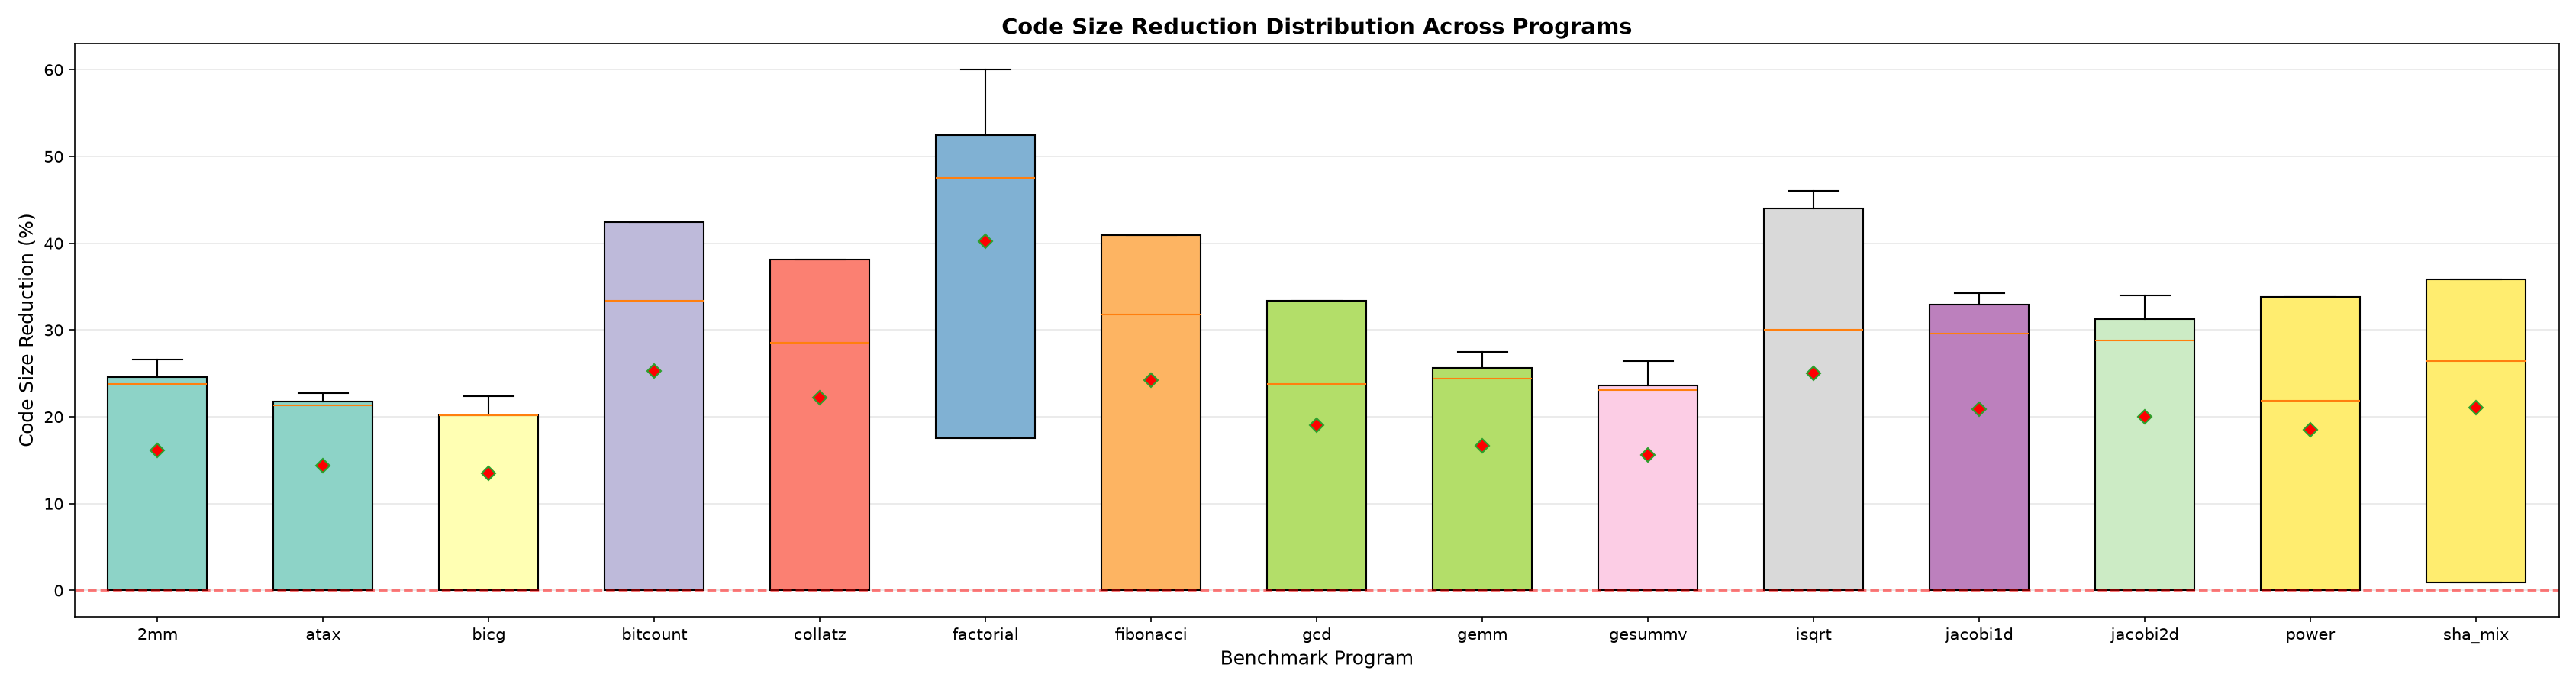
\includegraphics[width=0.88\textwidth]{fig/cross_program_box.png}
    \caption{Distribution of code-size reduction across all 720 orderings for each of the fifteen programs. Diamonds mark the mean. The lower whisker touches zero on every program except \texttt{factorial} and \texttt{sha\_mix}.}
    \label{fig:box}
\end{figure*}

\textbf{Equivalence classes.} Aggregated over the fifteen programs, the 720 orderings produce only nine distinct code-size outcomes (Table~\ref{tab:classes}). Each is a class of orderings that produce identical code on every program, determined entirely by the relative order of CF, CSE, CP, and DCE; the positions of SR and AS never change the instruction count. The $4! = 24$ relative orders each contain 30 orderings and map onto nine classes, so class sizes are multiples of 30. The cycle ratio varies within a class by less than 0.007, because SR rewrites $x \times 2$ as $x + x$ only when the literal is already in the instruction, which requires CF to have run first.

\begin{table}[!htbp]
\centering
\caption{The nine equivalence classes of orderings: geometric-mean normalized metrics over fifteen programs (baseline = 1.0)}
\label{tab:classes}
\renewcommand{\arraystretch}{1.05}
{\footnotesize
\setlength{\tabcolsep}{2.5pt}
\begin{tabular}{@{}clrccc@{}}
\toprule
\textbf{Class} & \textbf{Relative order (number of orders)} & \textbf{$n$} & \textbf{Size} & \textbf{Cyc.} & \textbf{Dyn.} \\
\midrule
1 & CF $\to$ CSE $\to$ CP $\to$ DCE & 30 & 0.643 & 0.795 & 0.768 \\
2 & CSE $\to$ CF $\to$ CP $\to$ DCE & 30 & 0.646 & 0.798 & 0.773 \\
3 & CF $\to$ CP, then CSE/DCE either way (2) & 60 & 0.651 & 0.801 & 0.782 \\
4 & CSE $\to$ CP $\to$ CF $\to$ DCE & 30 & 0.653 & 0.801 & 0.775 \\
5 & CP first, CF before DCE (3) & 90 & 0.660 & 0.804 & 0.785 \\
6 & CSE $\to$ CP $\to$ DCE $\to$ CF & 30 & 0.684 & 0.818 & 0.787 \\
7 & CP first, DCE before CF (3) & 90 & 0.691 & 0.821 & 0.797 \\
8 & CF before DCE before CP (4) & 120 & 0.753 & 0.839 & 0.815 \\
9 & DCE before both CF and CP (8) & 240 & 0.987 & 0.962 & 0.994 \\
\bottomrule
\end{tabular}
}
\end{table}

The table reads as rules that hold on every program. \textbf{DCE must follow CF and CP:} the eight relative orders in which DCE precedes both form class~9, a third of the space, with a size ratio of 0.987; on thirteen programs these 240 orderings leave the code unchanged, and the 1.3\% they achieve is the planted dead code in two programs. DCE removes only instructions whose results are unread, and in the baseline IR every temporary is read at least once; CF and CP are what make temporaries unread. \textbf{DCE after CF but before CP (class~8) loses a third of the benefit}, because CP is what makes copies such as \texttt{sum1 = t18} unread. \textbf{CF before CP beats CP before CF} (class~1 against class~5), because CF substitutes through single-assignment variables to a fixed point whereas CP substitutes within a basic block only. \textbf{CSE between CF and CP is best} (class~1 against classes~2 to~4): CSE matches more expressions after CF has replaced temporaries by literals, and the copies CSE creates shrink the code only if CP then propagates them and DCE deletes them. The marginal view agrees: averaged over all programs and orderings, the mean size ratio moves from 0.988 (DCE first) to 0.659 (DCE last), from 0.873 (CP last) to 0.681 (CP first), and from 0.841 (CF last) to 0.707 (CF first); CSE's position barely matters (0.789 against 0.793) and SR and AS have no effect (0.791 in both positions).

\subsection{Statistical Significance}
\label{sec:stats}
The Friedman test over the 24 relative orders, with the fifteen programs as blocks, rejects equivalence of orderings for all three metrics: code size $\chi^2(23) = 304.6$, $p = 5.3 \times 10^{-51}$, Kendall's $W = 0.88$; estimated cycles $\chi^2(23) = 296.0$, $p = 3.0 \times 10^{-49}$, $W = 0.86$; dynamic count $\chi^2(23) = 303.6$, $p = 8.5 \times 10^{-51}$, $W = 0.88$. A $W$ near 1 means the fifteen programs rank the orderings almost identically, which is the statistical form of the claim that the class structure is program-independent. The post-hoc comparison of class~1 against class~9 is an exact Wilcoxon signed-rank test on fifteen paired size ratios: $W = 0$, $p = 3.1 \times 10^{-5}$ (one-sided), $r = 1.00$, median paired difference 0.34 of the baseline size; class~1 is smaller on all fifteen programs, so the $p$-value is the smallest attainable with $n = 15$. These tests treat programs as the unit of replication; they establish that the ordering effect is not an artefact of one or two benchmarks, not that it holds for programs outside the suite.

\subsection{Trade-off Between Code Size and Execution Performance}
\label{sec:tradeoff}
Within this pass set there is no trade-off between the objectives at the level of classes: the class with the smallest code also has the lowest estimated cycles and the lowest dynamic count on all fifteen programs (Tables~\ref{tab:per_program} and~\ref{tab:classes}). Over the 10,800 optimized runs, Spearman's $\rho$ between normalized size and cycles is 0.79 and between size and dynamic count is 0.88; per program, the median $\rho$ between size and cycles is 1.00 and the minimum 0.88. The residual trade-off is within a class and comes from SR's position relative to CF: in class~1, orderings with SR after CF have a geometric-mean cycle ratio of 0.7950 and orderings with SR before CF have 0.7999, a 0.5\% difference with no change in size. The Pareto front of size against cycles is therefore short on every program. This is narrower than the size-versus-time conflict that POSET-RL reports for LLVM \cite{ref8}: the six passes here are all code-shrinking transformations, with no unrolling, inlining, or scheduling, which are the passes that trade size for speed, so the result is a property of this pass set rather than of phase ordering in general.

\subsection{Validation and Limitations}
\label{sec:validation}
Every one of the 10,800 optimized programs printed the same output as its baseline and terminated, as asserted by the benchmark driver and independently by the test suite. This is what allows the reductions to be read as optimization rather than accidental deletion: a soundness bug in any pass would appear as an output mismatch under some ordering, and one such bug in CSE was caught this way during development. As a further check, the baseline and class-1 IR of each program were lowered to RV32IM assembly: the reduction survives code generation with a geometric mean of 26.0\% (13.5\% on \texttt{bicg} to 50.4\% on \texttt{factorial}), smaller than the 35.7\% at the IR level because the back end has no register allocator.

Three limitations bound the claims. The cycle metric is a static cost model, not a hardware measurement; the dynamic instruction count is reported as a model-free second proxy, and the two agree in ranking ($\rho = 0.88$). The passes are block-local, so loop-carried copies such as \texttt{result = t3} survive in every loop of every benchmark; the measured reductions are a lower bound on what global data-flow versions would achieve, and the class structure may change in that setting. The benchmarks are adapted kernels at fixed, small problem sizes; results for unmodified MiBench and PolyBench sources, or for pass sets with loop and interprocedural transformations, are not established.

\section{Conclusion}
This paper studied the Phase Ordering Problem by exhaustive measurement on a small compiler in which six classical passes are block-local, independently reorderable units. All 720 orderings were applied to fifteen MiBench- and PolyBench-derived kernels, and every one of the 10,800 optimized programs was checked against its baseline output. The order of passes matters by a large factor: the best family of orderings reduces static code size by a geometric mean of 35.7\%, estimated cycles by 20.5\%, and executed instructions by 23.2\%, while the worst family, a third of all orderings, reduces code size by 1.3\% and leaves thirteen of the fifteen programs unchanged. The orderings collapse into nine equivalence classes fixed by the relative order of four passes, and the effect is consistent across programs (Friedman $p < 10^{-48}$, $W = 0.88$). The governing rule is that the passes which expose opportunities, Constant Folding and Copy Propagation, must run before the pass that consumes them, Dead Code Elimination, with Common Subexpression Elimination between them. On this pass set one relative order is optimal for every program and all three metrics at once; what varies is how many orderings reach it, from 30 to 360 of 720, with the array kernels least forgiving. Future work is to replace the cost model with cycles measured on RISC-V hardware through the existing back end, to add global passes and loop transformations and test whether the class structure survives, to evaluate unmodified MiBench and PolyBench sources, and to use the exhaustive results as ground truth for learned phase ordering.

% --- REFERENCES ---
\begin{thebibliography}{33}

\bibitem{ref21}
D. F. Bacon, S. L. Graham, and O. J. Sharp,
``Compiler transformations for high-performance computing,''
\textit{ACM Computing Surveys}, vol. 26, no. 4, pp. 345--420, 1994.
\url{https://doi.org/10.1145/197405.197406}

\bibitem{ref18}
K. D. Cooper, T. J. Harvey, and L. Torczon,
``Compiler-based code-improvement techniques,'' Rice University, 2002.
\url{https://www.cs.tufts.edu/~nr/cs257/archive/keith-cooper/survey.pdf}

\bibitem{ref19}
P. Kulkarni \textit{et al.},
``Fast searches for effective optimization phase sequences,''
\textit{ACM SIGPLAN Notices}, vol. 39, no. 6, pp. 171--182, 2004.
\url{https://doi.org/10.1145/996893.996863}

\bibitem{ref1}
J. Liu \textit{et al.},
``Efficient compiler optimization by modeling passes dependence,''
\textit{CCF Trans. High Performance Computing}, 2024.
\url{https://doi.org/10.1007/s42514-024-00197-9}

\bibitem{ref2}
R. Han and H. Kim,
``Exponentially expanding the phase-ordering search space via dormant information,''
in \textit{Proc. ACM SIGPLAN Int. Conf. Compiler Construction (CC)}, 2024.
\url{https://doi.org/10.1145/3640537.3641582}

\bibitem{ref16}
C. Lattner and V. Adve,
``LLVM: A compilation framework for lifelong program analysis and transformation,''
in \textit{Proc. Int. Symp. Code Generation and Optimization (CGO)}, 2004.
\url{https://doi.org/10.1109/CGO.2004.1281665}

\bibitem{ref32}
M. R. Guthaus, J. S. Ringenberg, D. Ernst, T. M. Austin, T. Mudge, and R. B. Brown,
``MiBench: A free, commercially representative embedded benchmark suite,''
in \textit{Proc. IEEE Int. Workshop on Workload Characterization (WWC-4)}, 2001.
\url{https://doi.org/10.1109/WWC.2001.990739}

\bibitem{ref31}
L.-N. Pouchet,
``PolyBench/C: The polyhedral benchmark suite,'' version 4.2, 2016.
\url{https://web.cse.ohio-state.edu/~pouchet.2/software/polybench/}

\bibitem{ref4}
F. Huemer, D. Leopoldseder, A. Prokopec, R. Mosaner, and H. M\"ossenb\"ock,
``Taking a closer look: An outlier-driven approach to compilation-time optimization,''
in \textit{Proc. 38th European Conf. Object-Oriented Programming (ECOOP)}, 2024.
\url{https://doi.org/10.4230/LIPIcs.ECOOP.2024.20}

\bibitem{ref8}
S. Jain \textit{et al.},
``POSET-RL: Phase ordering for optimizing size and execution time using reinforcement learning,''
in \textit{Proc. IEEE Int. Symp. Performance Analysis of Systems and Software (ISPASS)}, 2022.
\url{https://doi.org/10.1109/ISPASS55109.2022.00012}

\bibitem{ref12}
Q. Huang \textit{et al.},
``AutoPhase: Compiler phase-ordering for high-level synthesis,'' arXiv:2003.00671, 2020.
\url{https://doi.org/10.48550/arXiv.2003.00671}

\bibitem{ref15}
A. H. Ashouri, A. Bignoli, G. Palermo, C. Silvano, S. Kulkarni, and J. Cavazos,
``MiCOMP: Mitigating the compiler phase-ordering problem using optimization subsequences and machine learning,''
\textit{ACM Trans. Architecture and Code Optimization}, vol. 14, no. 3, pp. 1--28, 2017.
\url{https://doi.org/10.1145/3124452}

\bibitem{ref9}
S. VenkataKeerthy \textit{et al.},
``IR2Vec: LLVM IR based scalable program embeddings,''
\textit{ACM Trans. Architecture and Code Optimization}, vol. 17, no. 4, 2020.
\url{https://doi.org/10.1145/3418463}

\bibitem{ref17}
A. H. Ashouri, A. Bignoli, G. Palermo, and C. Silvano,
``Predictive modeling methodology for compiler phase-ordering,''
in \textit{Proc. PARMA-DITAM Workshops}, 2016, pp. 7--12.
\url{https://doi.org/10.1145/2872421.2872424}

\bibitem{ref22}
M. Zhu and D. Hao,
``Compiler auto-tuning via critical flag selection,''
in \textit{Proc. IEEE/ACM Int. Conf. Automated Software Engineering (ASE)}, 2023.
\url{https://doi.org/10.1109/ASE56229.2023.00209}

\bibitem{ref28}
H. Liu, J. Xu, S. Chen, and T. Guo,
``Compiler optimization parameter selection method based on ensemble learning,''
\textit{Electronics}, vol. 11, no. 15, 2022.
\url{https://doi.org/10.3390/electronics11152452}

\bibitem{ref29}
C. Shewale, S. B. Shinde, Y. B. Gurav, R. J. Patil, and S. U. Kadam,
``Compiler optimization prediction with new self-improved optimization model,''
\textit{Int. J. Advanced Computer Science and Applications}, vol. 14, no. 2, 2023.
\url{https://doi.org/10.14569/IJACSA.2023.0140267}

\bibitem{ref20}
R. Nobre, L. G. A. Martins, and J. M. P. Cardoso,
``A graph-based iterative compiler pass selection and phase ordering approach,''
in \textit{Proc. 17th ACM SIGPLAN/SIGBED Conf. Languages, Compilers, Tools, and Theory for Embedded Systems (LCTES)}, 2016, pp. 21--30.
\url{https://doi.org/10.1145/2907950.2907959}

\bibitem{ref26}
R. Han and H. Kim,
``Exponentially expanding the compiler phase-ordering problem's search space through the learning of dormant information,'' OpenReview preprint, 2023.
\url{https://openreview.net/pdf?id=frjDLUebFY}

\bibitem{ref25}
Y. Chen, H. Chen, Y. Yao, P. Yu, F. Xu, and X. Ma,
``Exploiting booster pass chain for compiler phase ordering,''
in \textit{Proc. 16th Int. Conf. Internetware}, 2025, pp. 175--185.
\url{https://doi.org/10.1145/3755881.3755899}

\bibitem{ref3}
Y. Wang, H. Chen, and K. Wang,
``Beyond the phase ordering problem: Finding the globally optimal code with respect to optimization phases,'' arXiv:2410.03120, 2024.
\url{https://doi.org/10.48550/arXiv.2410.03120}

\bibitem{ref23}
S. Kloibhofer,
``Run-time data analysis to drive compiler optimizations,''
in \textit{Companion Proc. ACM SIGPLAN SPLASH}, 2021, pp. 9--12.
\url{https://doi.org/10.1145/3484271.3484974}

\bibitem{ref24}
A. Pe\v{c}im\'{u}th, D. Leopoldseder, and P. T\r{u}ma,
``Diagnosing compiler performance by comparing optimization decisions,''
in \textit{Proc. 20th ACM SIGPLAN Int. Conf. Managed Programming Languages and Runtimes (MPLR)}, 2023, pp. 47--61.
\url{https://doi.org/10.1145/3617651.3622994}

\bibitem{ref7}
J. Zhao \textit{et al.},
``Leveraging compilation statistics for compiler phase ordering,''
in \textit{Proc. IEEE Int. Parallel and Distributed Processing Symp. (IPDPS)}, 2025.
\url{https://doi.org/10.1109/IPDPS64566.2025.00054}

\bibitem{ref27}
A. H. Ashouri, S. S. G. Bagi, K. Satheeskumar, T. Srikanth, J. Zhao, I. Saidoun, Z. Wang, B. Chan, and T. S. Czajkowski,
``Protean compiler: An agile framework to drive fine-grain phase ordering,'' arXiv:2602.06142, 2026.
\url{https://doi.org/10.48550/arXiv.2602.06142}

\bibitem{ref30}
R. Koitz-Hristov, F. Mandl, and F. Wotawa,
``VisOpt: Visualization of compiler optimizations for computer science education,''
in \textit{Proc. 56th ACM Technical Symp. Computer Science Education (SIGCSE TS)}, 2025, pp. 603--609.
\url{https://doi.org/10.1145/3641554.3701832}

\bibitem{ref33}
P. J. Fleming and J. J. Wallace,
``How not to lie with statistics: The correct way to summarize benchmark results,''
\textit{Communications of the ACM}, vol. 29, no. 3, pp. 218--221, 1986.
\url{https://doi.org/10.1145/5666.5673}

\bibitem{ref5}
H. Ahmed, M. F. Hyder, M. F. ul Haque, and P. C. Santos,
``Exploring compiler optimization space for control flow obfuscation,''
\textit{Computers \& Security}, 2024.
\url{https://doi.org/10.1016/j.cose.2024.103704}

\bibitem{ref6}
A. Schmitz \textit{et al.},
``Parallel pattern compiler for automatic global optimizations,''
\textit{Parallel Computing}, 2024.
\url{https://doi.org/10.1016/j.parco.2024.103112}

\bibitem{ref10}
M. Camilli, A. Janes, and B. Russo,
``Automated test-based learning and verification of performance models for microservices systems,''
\textit{Journal of Systems and Software}, vol. 187, 2022.
\url{https://doi.org/10.1016/j.jss.2022.111225}

\bibitem{ref11}
S. Zhang, X.-W. Guo, C. Li, Y. Liu, S. Fan, R. Zhao, and C. Yang,
``A large scale parallel fluid-structure interaction computing platform for simulating structural responses to a detonation shock,''
\textit{Software: Practice and Experience}, vol. 53, no. 1, pp. 211--240, 2023.
\url{https://doi.org/10.1002/spe.3051}

\bibitem{ref13}
M. Tao,
``Semantic ontology enabled modeling, retrieval and inference for incomplete mobile trajectory data,''
\textit{Future Generation Computer Systems}, vol. 145, pp. 1--11, 2023.
\url{https://doi.org/10.1016/j.future.2023.03.012}

\bibitem{ref14}
F. Fernandes dos Santos, L. Carro, F. Vella, and P. Rech,
``Assessing the impact of compiler optimizations on GPUs reliability,''
\textit{ACM Trans. Architecture and Code Optimization}, vol. 21, no. 2, 2024.
\url{https://doi.org/10.1145/3638249}

\end{thebibliography}

\end{document}
